\documentclass[]{article}


% included packages
% used to include images
\usepackage{graphicx}
% used to add caption to figures, tables, etc.
\usepackage{caption}
% used to add captions to subfigures
\usepackage{subcaption}
% make tables span over more than one page
\usepackage{longtable}
% to avoid the use of static table widths
\usepackage{tabularx}
% add hyperlinks in the texts
\usepackage{hyperref}
% add tick an cross
\usepackage{pifont}

% Create simple commands to create ticks and crosses
\newcommand{\tick}{\ding{51}}
\newcommand{\cross}{\ding{55}}

% correct bad hyphenation here
\hyphenation{}

% remove heading of bibliography as it is located in a subsection with text
\makeatletter
\renewenvironment{thebibliography}[1]{%
%     \section*{\refname}%
%      \@mkboth{\MakeUppercase\refname}{\MakeUppercase\refname}%
      \list{\@biblabel{\@arabic\c@enumiv}}%
           {\settowidth\labelwidth{\@biblabel{#1}}%
            \leftmargin\labelwidth
            \advance\leftmargin\labelsep
            \@openbib@code
            \usecounter{enumiv}%
            \let\p@enumiv\@empty
            \renewcommand\theenumiv{\@arabic\c@enumiv}}%
      \sloppy
      \clubpenalty4000
      \@clubpenalty \clubpenalty
      \widowpenalty4000%
      \sfcode`\.\@m}
     {\def\@noitemerr
       {\@latex@warning{Empty `thebibliography' environment}}%
      \endlist}
\makeatother


\begin{document}

% paper title
% can use linebreaks \\ within to get better formatting as desired
\title{Need4Feed: \\
Software Requirement Specification\\
by BIT}


% author names and affiliations
% use a multiple column layout for up to three different
% affiliations
\author{Brian Pohl\\
Student ID: 9100920124\\
\texttt{enzothebaker8@gmail.com}
\and
Iker Trun\\
Student ID: 9101920127\\
\texttt{iktrun@gmail.com}
\and
Thomas Ingvarsson\\
Student ID: 9093920122\\
\texttt{ingvarsson.thomas@sillys.se}
}


% make the title area
\maketitle


\begin{abstract}
Nowadays the most common form of communication between people all over the world is taking place on the Internet, or specifically through media such as social networks, forums, and blogs. Blogging has become more and more popular during over the last ten years. The blog is an information sharing tool that allows the user to write about anything that is interesting for him or her and potentially for others with common interests. Through low-maintenance web-based solutions there is also almost no technical knowledge required, compared to more complex web pages, for a user to start and maintain a blog. On the other side taking in information has become just as easy. In today's society everybody has a smartphone with an Internet connection, keeping them online at all time. Users are able to be online on social networks, read forums or follow blogs whenever they like to. The idea of joining the wide assortment of topics a user might find interesting, in a more convenient, more easily consumable form has become attractive for users that would like to have all this information organized in one single location, such as in an application on their smartphones.
\end{abstract}


\section*{Revision History}
\begin{center}
    \begin{tabularx}{\linewidth}{ | l | l | X | l |}
    \hline
    \textbf{Version} & \textbf{Date} & \textbf{Description} & \textbf{Author}\\ \hline
    0.1 & 09-Oct-2012 & First draft. & T. Ingvarsson\\ \hline
    0.11 & 09-Oct-2012 & Added Revision History and Table of Contents. & T. Ingvarsson\\ \hline
    0.12 & 09-Oct-2012 & Detailed Requirements table has been remade into a multi-page table. & T. Ingvarsson\\ \hline
    0.13 & 14-Oct-2012 & Stream-lined the abstract and introduction to not have too much redundancy. & T. Ingvarsson\\ \hline
    0.14 & 15-Oct-2012 & Software Interfaces is rewritten as pure requirements that do not imply how it should be solved. & T. Ingvarsson \\ \hline
    0.15 & 15-Oct-2012 & Major overhaul of User Interfaces. Simplified and removed unnecessary descriptions. To strict requirements are removed at this stage. & T. Ingvarsson\\ \hline
    0.16 & 15-Oct-2012 & Major overhaul of Product Features. Added a use case diagram including a better overview of the features as well as a list of actors to the system. & T. Ingvarsson\\ \hline
    0.17 & 16-Oct-2012 & Simplified the System Features section by removing the functional requirements of every subsection, this will be covered in the detailed requirement list anyway. Removed feed list and all with it, is not a feature requirement.  Removed subsection Manage Categories as this is covered in Manage Feeds. & T. Ingvarsson\\ \hline
    0.18 & 19-Oct-2012 & Added References. & T. Ingvarsson\\ \hline
    0.19 & 23-Oct-2012 & Added Software Quality Attributes to Other Non-functional Requirements. & T. Ingvarsson\\ \hline
    0.20 & 23-Oct-2012 & Updated use case diagram with more sub-features. Updated System Features to match the use case diagram. & T. Ingvarsson\\ \hline
    % copy the last line before adding the new revision.
    \end{tabularx}
    
    % new page of revision history
    \begin{tabularx}{\linewidth}{ | l | l | X | l |}
    \hline
    \textbf{Version} & \textbf{Date} & \textbf{Description} & \textbf{Author}\\ \hline
    0.21 & 24-Oct-2012 & Update the Detailed Requirement list to match the rest of the updates. & T. Ingvarsson\\ \hline
    0.22 & 27-Oct-2012 & Added new features; Share Post, Import Feed(s), Export Feed(s), Find Similar Feed(s). Changed so it should handle multiple kinds of sources, not just RSS. & T. Ingvarsson\\ \hline
    0.30 & 21-Nov-2012 & Added comparison table of the most popular readers existing on the Google Play Store to clarify the differences. & T. Ingvarsson\\ \hline
    0.31 & 26-Nov-2012 & Added a system feature; gather and display statistics. Also updated the deadlines mentioned under project constraints. & T. Ingvarsson\\ \hline
     &  &  & \\ \hline
    % copy the last line before adding the new revision.
    \end{tabularx}
\end{center}


\setcounter{tocdepth}{2}
\tableofcontents


\section{Introduction}


\subsection{Purpose}
The purpose of this document is to specify a software for Android users enabling the functionality to gather, organize and read feeds, regardless of if it is a RSS\cite{rss-spec}, ATOM\cite{atom}, Podcasts or social medium feed. Furthermore, this requirement specification will act as base for the specification which in turn will be the base of the design document. This will be the first release of the mentioned software which is completely standalone in the sense that it is not part of a larger system.


\subsection{Intended Audience and Reading Suggestions}
The intended audience for this document are those with an engineering background interested in this project, whether it be the actual teacher assigning this project to the project group, one of the group members or an actual user wanting to know more about the product or continue development. Due to the small size of the actual product I would recommend all readers to read the whole document from start to finish. However to understand the major features, section~\ref{sec:overall_description} will do. If one is only interested in the actual requirements they are listed in section~\ref{sec:detailed_requirements}, Detailed Requirements. A section in which all requirements are listed with their ID, short description, priority and source.


\subsection{Project Scope}
Nowadays the most common form of communication between people all over the world is taking place on the Internet, or specifically through media such as social networks, forums, and blogs. Blogging has become more and more popular during over the last ten years. The blog is an information sharing tool that allows the user to write about anything that is interesting for him or her and potentially for others with common interests. Through low-maintenance web-based solutions there is also almost no technical knowledge required, compared to more complex web pages, for a user to start and maintain a blog. On the other side taking in information has become just as easy. In today's society everybody has a smartphone with an Internet connection, keeping them online at all time. Users are able to be online on social networks, read forums or follow blogs whenever they like to. The idea of joining the wide assortment of topics a user might find interesting, in a more convenient, more easily consumable form has become attractive for users that would like to have all this information organized in one single location, such as in an application on their smartphones.

The development team for this software project has set out to minimize the clutter that comes along with following many different sources, while simultaneously being able to organize the material in great depth. The goal of the program is to minimize time spent ineffectively trying to manage multiple sources and maximize the content available for the user.

Today there exist several similar solutions; web-based such as \textit{Google Reader}\cite{g-reader}, desktop clients such as \textit{Reeder}\cite{reeder} and smartphone applications such as \textit{Feedly}\cite{feedly}. What this software will offer to its users compared to the already existing solutions is a minimalistic interface with low overhead but still capable of giving the full-fledged feed experience, without relying on a web-based service such as \textit{Google Reader}. An experience including adding your favorite feeds, categorizing them and keeping track of the latest posts. By including the possibility to follow social mediums, such as \textit{Facebook} or \textit{Twitter}, along side your regular feeds the product distinguishes from its competition. 
\begin{table}
\begin{center}
\begin{tabularx}{1.05\linewidth}{X*{6}{c}}
Feature & Feedly & FeedR & Pulse News & gReader & Need4Feed \\
\hline \\
Supports \textit{RSS}, \textit{ATOM}, and \textit{Podcast} & \tick & \tick & \tick & \tick & \tick\\
Supports \textit{Facebook} and \textit{Twitter} & & & \tick & & \tick\\
Supports \textit{Youtube} and \textit{Tumblr} & \tick & & \tick & & \\
Supports \textit{Digg}, \textit{Flickr}, \textit{PicPlz}, \textit{Reddit}, and \textit{Vimeo} & & & \tick & & \\
Categorize Feeds & \tick & \tick & \tick & \tick & \tick \\
Store Locally & \tick & \tick & \tick & \tick & \tick \\
Share to Social Networks & \tick & \tick & \tick & \tick & \tick \\
Integrate with Google Reader & \tick & \tick & \tick & \tick & \\
Require Account & \tick & \tick & \tick & \tick & \\
Suggest Feeds & \tick & & \tick & & \tick \\
Multi-Language & \tick & & \tick & & \\
Personalize with Themes & \tick & \tick & \tick & \tick & \\
Open-source & & & & & \tick \\
\end{tabularx}
\caption{Supported Features of The Most Popular RSS Readers}\label{tab:support_list}
\end{center}
\end{table}

Seen in table~\ref{tab:support_list} are the four most popular \textit{RSS} Readers listed along side with this product. Compared are the main features of each product to visualize where this product succeeds compared to its competition. First thing that can be noticed in the table is that all readers have the same standard support of sources while \textit{Pulse News} plays in its own division with a massive list of supported sources. Here does the product land in the middle, supporting the most popular sources without bloating with less used or popular sources the way one could discuss that \textit{Pulse News} does. Beyond that one can also observe that the product requires no integration with \textit{Google Reader} as mentioned earlier, actually no account all is required to use the product removing any ties otherwise created using one of the more popular choices. The last but not least difference, one could even consider it being the most important one, is that the product is open-source, something the more popular choices are not.

The user of the suggested solution is anyone with a smartphone wanting to organize and follow their favorite feeds through a software that is convenient and approachable. The user should be able to go to the software whenever they have downtime or the need of the latest information.


\subsection{Project Constraints}
The most pressing constraint of the project is that it must be completed within a strict time frame where there are deadlines for multiple milestones. These milestones are:
\begin{description}
  \item[9th October] Requirement Analysis: Software Requirements Specification
  \item[23rd October] Specification: Structured system/Object-oriented analysis
  \item[22th November] Design/Implementation: Architecture design and Source code/Testing
  \item[7th December] Demo: Presentation/Installation guide
\end{description}
Another constraint is the limited development team, consisting only of the project group of three people. 


\subsection{Definitions, acronyms and abbreviations}
Below is a list of definitions, acronyms and abbreviations referenced in this document, sorted after appearance.

\begin{description}
  \item[Android] \hfill \\
  A mobile operating system developed by Google
  \item[RSS] \hfill \\
  \textbf{R}ich \textbf{S}ite \textbf{S}ummary
  \item[ATOM] \hfill \\
  The Atom Syndication Format is an XML language used for web feeds
  \item[Podcast] \hfill \\
  A multimedia digital file made available on the Internet for downloading
  \item[Google Reader] \hfill \\
  Google Reader is a Web-based aggregator, capable of reading Atom and RSS feeds online or offline
  \item[Reeder] \hfill \\
  A Google Reader client for Mac
  \item[Feedly] \hfill \\
  A Google Reader client for Chrome, iOS, Android and Kindle
  \item[Facebook] \hfill \\
  A social networking website launched in February 2004
  \item[Twitter] \hfill \\
  An online social networking service and microblogging service
  \item[TBD] \hfill \\
  \textbf{T}o \textbf{B}e \textbf{D}eclared
  \item[Froyo] \hfill \\
  Version 2.2 of the Android operating system
  \item[Ice Cream Sandwich] \hfill \\
  Version 4.1 of the Android operating system
\end{description}


\subsection{References}
In this section is a list of all documents referenced throughout the rest of this document.

\bibliography{ref}
\bibliographystyle{unsrt}


\section{Overall Description}
\label{sec:overall_description}

\subsection{Product Perspective}
The product to be is a new open-source feed reader, with no predecessors, that will compete with existing solutions on the market by offering an low-overhead and minimalistic interface without the need of a web-based back-end. The goal is to give users a simple but powerful feed reading solution.

\subsection{Product Features}
\label{sec:product_features}
\begin{figure}[hbt]
\centering
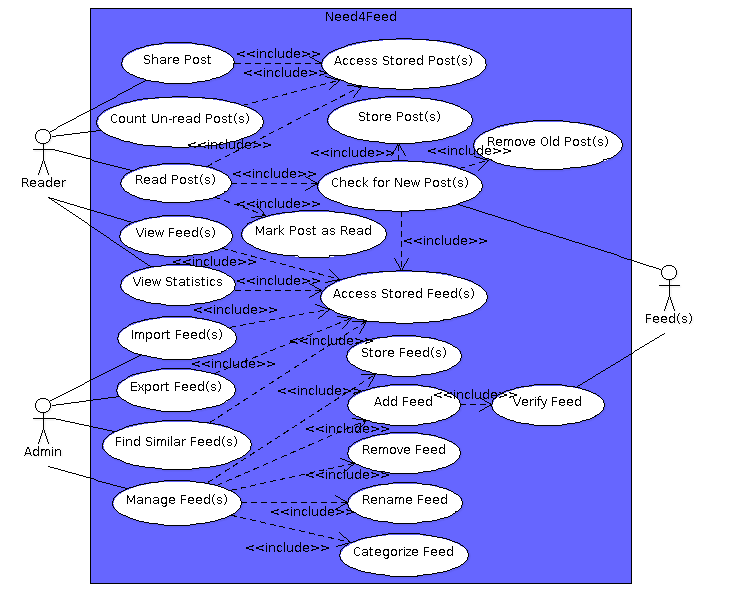
\includegraphics[width=\textwidth]{./images/UseCaseDiagramGeneralFull.png}
\caption{Complete use case of the major features}
\label{fig:use_case}
\end{figure}
The product's use case diagram is shown in figure~\ref{fig:use_case}, where actors, major features and included sub-features are displayed. The overall feature can be described as a feed library where the user can organize feeds as well as view posts. The actors of the product are Reader and Admin, which are subsets of User, as well as Feed(s). Feed(s) are not a person but still an actor to the product as it provides data.\\ \\
The major features of the product are:

\begin{itemize}
  \item Share Post
  \item Count Un-read Post(s)  
  \item Read Post(s)
  \item View Feed(s)
  \item Import Feed(s)
  \item Export Feed(s)
  \item Find Similar Feed(s)
  \item Manage Feed(s)
\end{itemize}
Underneath the major features are a set of sub-features to describe the flow of the product.\\ \\
The major user interfaces are:

\begin{itemize}
  \item View Categories
  \item View Feeds
  \item View Posts
  \item View Post
\end{itemize}
The product shall include these four user interfaces to enable the user to utilize all the major features of the product.


\subsection{Operating Environment}
The environment for the product shall be Android\cite{android}, which is an operating system for touchscreen mobile devices. The product shall be supported for Android version 2.2, \textit{Froyo}, up to 4.1, \textit{Ice Cream Sandwich}. The product shall comply the hardware requirements that are required by the specified Android versions. 


\subsection{User Documentation}
To complement the product a user manual shall be created. This manual shall contain common user scenarios as well as descriptions of all options available throughout the user interface. An optional addition would be a developer’s guide to encourage outsiders to get involved.




\section{System Features}
In this section are the major features mentioned in section~\ref{sec:product_features} described, sub-features are handled within each parent feature. 

\subsection{Share Post}
The product shall be able to share a post and its content over a social medium. This feature is an optional feature for the product and has low priority.


\subsubsection{Stimulus/Response Sequences}
User triggered:
\begin{itemize}
  \item Share Post - Compile a post containing the post's address and a user comment and send to a social medium.
\end{itemize}
System triggered:
\begin{itemize}
  \item Access Stored Post(s) - Access the address of a locally stored post.
\end{itemize}


\subsection{Count Un-read Post(s)}
The product shall be able to present the amount of un-read posts stored locally. This feature is an optional feature for the product and has medium priority.


\subsubsection{Stimulus/Response Sequences}
User triggered:
\begin{itemize}
  \item Count Un-read Post(s) - The amount of un-read post(s) should be presented to the user in the appropriate view.
\end{itemize}
System triggered:
\begin{itemize}
  \item Access Stored Post(s) - Access and check the read status of all locally stored post(s).
\end{itemize}


\subsection{Read Post(s)}
The product shall give the user the ability to Read either several posts, by their headers, or a single post with all of its content. To make sure that the user has the latest posts available the product shall check for new posts, and if any store them locally. To preserve memory shall the product only store a certain amount of posts per feed, once this limit has been reached the product shall remove the oldest posts. The posts presented to the user shall be stored locally and when read they should be marked as read. This feature, along with its sub-features, are key features for the product and have high priority.


\subsubsection{Stimulus/Response Sequences}
User triggered:
\begin{itemize}
  \item Read posts - List several posts in an appropriate view where the header of several posts can be read at the same time.
  \item Read post - Display a post, both the header and the content , in an appropriate view.
\end{itemize}
System triggered:
\begin{itemize}
  \item Check for New Post(s) - Fetch all the latest posts on start-up or when a new feed has been added.
  \item Access Stored Feed(s) - To determine where the posts should be fetched from the feed(s) has to be loaded from local storage.
  \item Store Post(s) - Store all posts along with its attributes: date, parent feed and read status.
  \item Remove Old Post(s) - Remove old posts either on startup to lower memory usage, combined with removal of feed or removal of read posts.
  \item Access Stored Post(s) - Load a stored post to avoid unnecessary fetch.
  \item Mark Post as Read - Mark a post as read when it has been viewed by an user.
\end{itemize}


\subsection{View Feed(s)}
The product shall give the user the ability to View feeds. This feature is a key feature for the product and has high priority.


\subsubsection{Stimulus/Response Sequences}
User triggered:
\begin{itemize}
  \item View Feed(s) - List all added feeds in an appropriate view where multiple feeds are visible at the same time.
\end{itemize}
System triggered:
\begin{itemize}
  \item Access Stored Feed(s) - Access locally stored feeds to be able to list them.
\end{itemize}


\subsection{View Statistics}
The product should give the user the ability to View statistics gathered during the usage of the product. The statistics shall include how much time the user spends reading each post, viewing a feed, or category. It should also record the amount of re-reads of posts, amount of un-read posts marked as read, and read posts per day, week, month or forever. The statistics should be presented in such a way that the relevant information is shown. This feature is an optional feature for the product and has low priority.


\subsubsection{Stimulus/Response Sequences}
User triggered:
\begin{itemize}
  \item View Statistics - Lists all statistics recorded by the product since install.
\end{itemize}
System triggered:
\begin{itemize}
  \item Access Stored Feed(s) - Access locally stored feeds to accesses stored statistics gathered throughout the use.
\end{itemize}


\subsection{Import/Export Feed(s)}
The product shall be able to import or export all feeds in a standardized way to, or from, other feed services. This feature is an optional feature for the product and has low priority.


\subsubsection{Stimulus/Response Sequences}
User triggered:
\begin{itemize}
  \item Import/Export Feed(s) - Combine all existing feed(s) into a standardized file format to be imported elsewhere. Import  is a way to mass-add feed(s).
\end{itemize}
System triggered:
\begin{itemize}
  \item Access Stored Feed(s) - Access locally stored feed(s).
\end{itemize}


\subsection{Find Similar Feed(s)}
The product shall be able to look for similar feed(s) and present them to the user. This feature is an optional feature for the product and has low priority.


\subsubsection{Stimulus/Response Sequences}
User triggered:
\begin{itemize}
  \item Find Similar Feed(s) - Look for similar feeds by the use of online databases.
\end{itemize}
System triggered:
\begin{itemize}
  \item Access Stored Feed(s) - Access locally stored feed(s) to use as search term.
\end{itemize}


\subsection{Manage Feed(s)}
The product shall give the user the ability to Add, Remove, Rename and Categorize feeds. Adding a feed shall require the product to first verify that the feed exists. The product shall store all feeds locally so that they can be accessed at a later time again. This feature, along with its sub-features, are key features for the product and have high priority.


\subsubsection{Stimulus/Response Sequences}
User triggered:
\begin{itemize}
  \item Add, Remove, Rename, Categorize - Options that should be accessible through the user interface in the appropriate view.
\end{itemize}
System triggered:
\begin{itemize}
  \item Categorize - All feeds should as default be categorized, either when added without category or at removal of category, to category \textit{Uncategorized}. This will guarantee that all feeds have a category assigned.
  \item Verify Feed - The product shall verify that the RSS feed exists to complete an add feed operation.
  \item Store Feed(s) - All feeds should be stored so that they can be accessed at a later time again.
\end{itemize}


\section{System Interface}


\subsection{User Interfaces}
The product shall provide a set of views enabling the user to all system features. 

\subsubsection{Main View}
The product shall be able to list all categories in alphabetic order, clicking on a category shall take the user to the \textit{Feeds View} for that specific category. The view shall include the following options:

\begin{itemize}
  \item Add category
  \item Remove category
  \item Add feed
  \item Fetch posts
\end{itemize}
The first entry in the list should be a \textit{View all\ldots} button that should show the latest posts from all feeds in all categories. The last entry in the list should be a \textit{Add Category\ldots} button.


\subsubsection{Category View}
The product shall be able to list all feeds for a specific category in alphabetic order, clicking on a feed shall take the user to the \textit{Posts View} for that specific feed. The view shall include the following options:

\begin{itemize}
  \item Add feed
  \item Remove feed
  \item Remove active category
  \item Fetch posts
\end{itemize}
The first entry in the list should be a \textit{View All\ldots} button that should show the latest posts from all feeds in the specific category. The last entry in the list should be a \textit{Add Feed\ldots} button.


\subsubsection{Feed View}
The product shall be able to list the latest posts for a specific feed in a latest first order. Clicking on a post shall take the user to the \textit{Post View} for that specific post. The posts shall be displayed with their heading. The view shall include the following options:

\begin{itemize}
  \item Mark all posts as read/unread
  \item Remove active feed
  \item Fetch posts
\end{itemize}
The last entry in the list should be a \textit{Older Posts\ldots} button that should fetch older posts to show.


\subsubsection{Post View}
The product shall be able to display a specific post and all of its content. The view should enable sliding; sliding the screen to the right should show a older post, while sliding to the left should show a newer post. 


\subsection{Software Interfaces}


\subsubsection{Internet}
The product shall require access to Internet so that RSS feeds can be accessed and posts be downloaded. RSS feeds shall be accessed through either HTTP or FTP.


\subsubsection{External Memory}
The product should be able to store settings, feed lists and posts on an external memory. It should be able to both store and remove files. 


\subsubsection{Background Task}
The product should periodically update; download new posts and delete old ones. If the product's main interface is active it shall make sure that an opened post is not deleted.


\subsubsection{Notification Bar}
The product should be able to notify the user that there are new posts through the notification bar. It should also show the amount of un-read posts.


\section{Other Non-functional Requirements}


%\subsection{Performance Requirements}
%Performance Requirements text here. Response times/refresh rate, Processing times


\subsection{Security Requirements}
For the product to work properly it will require permission from the user for certain features according to Android\cite{android-perm}.\\ \\
Android user permissions required:
\begin{itemize}
  \item Full Internet Access - To access and download RSS feeds.
\end{itemize}
Android user permissions that depends on optional features:
\begin{itemize}
  \item Modify/Delete SD Card Content - Enables storage of settings, feed list and posts on SD card.
  \item Modify Global System Settings - Enables the use of notifications.
\end{itemize}


\subsection{Software Quality Attributes}
In this subsection are software quality requirements that are non-functional listed.
\begin{description}
  \item[Availability] \hfill \\
The product shall be available at all time, even without Internet access.
  \item[Flexibility] \hfill \\
Functionality should be possible to add without affecting the current functionality.
  \item[Reliability] \hfill \\
The product should not lose performance due to too much content in either the amount of feeds, posts or the content within one post.
  \item[Scalability] \hfill \\
The product shall be able to store and handle feeds and posts in such a way that only the actual storage size in memory restricts. The product should be able to handle throughput from unlimited amounts of feeds without preventing the user accessing already downloaded posts.
  \item[Usability] \hfill \\
The user shall without reading a manual be able to add, remove, categorize feeds. Beyond that the user shall also be able to, again without reading a manual, view all feeds, view feeds of a certain category, view posts of a certain feed and view individual posts.
\end{description}



\section{Detailed Requirements}
\label{sec:detailed_requirements}
In table~\ref{tab:detailed_requirements} all the requirements are listed with an ID, short description and priority. The different ID categories are:
\begin{description}
  \item[P] Post
  \item[F] Feed
  \item[U] User Interface
  \item[I] Interface
  \item[S] Security
  \item[Q] Quality
\end{description}

\begin{center}
\begin{longtable}{ | l | p{8cm} | l | }
\caption{List of Detailed Requirements}
\label{tab:detailed_requirements} \\

\hline \multicolumn{1}{|c|}{\textbf{ID}} & \multicolumn{1}{c|}{\textbf{Description}} & \multicolumn{1}{c|}{\textbf{Priority}}  \\ \hline 
\endfirsthead

\multicolumn{3}{c}%
{{\bfseries \tablename\ \thetable{} -- continued from previous page}} \\
\hline \multicolumn{1}{|c|}{\textbf{ID}} & \multicolumn{1}{c|}{\textbf{Description}} & \multicolumn{1}{c|}{\textbf{Priority}} \\ \hline 
\endhead

\hline \multicolumn{3}{|r|}{{Continued on next page}} \\ \hline
\endfoot

\hline
\endlastfoot

    P-1 & Check for new Post(s) & High Priority \\ \hline
    P-2 & Store Post(s) & High Priority \\ \hline
    P-3 & Remove Old Post(s) & High Priority \\ \hline
    P-4 & Access Stored Post(s) & High Priority \\ \hline
    P-5 & Mark Post as Read & Medium Priority \\ \hline
    P-6 & Count Un-read Post(s) & Medium Priority \\ \hline
    P-7 & Share Post & Low Priority \\ \hline
     &  &  \\ \hline
    F-1 & Add Feed & High Priority \\ \hline
    F-2 & Remove Feed & High Priority \\ \hline
    F-3 & Rename Feed & High Priority \\ \hline
    F-4 & Categorize Feed & High Priority \\ \hline
    F-5 & Verify Feed & High Priority \\ \hline
    F-6 & Store Feed(s) & High Priority \\ \hline
    F-7 & Access Stored Feed(s) & High Priority \\ \hline
    F-8 & Export Feed(s) & Low Priority \\ \hline
    F-9 & Import Feed(s) & Low Priority \\ \hline
    F-10 & Find Similar Feed(s) & Low Priority \\ \hline
     &  &  \\ \hline
    U-1 & Present the Amount of Un-read Post(s) & Medium Priority \\ \hline
    U-2 & Present a List of Post(s) & High Priority \\ \hline
    U-3 & Present a Single Post with Header and Content & High Priority \\ \hline
    U-4 & Present a List of Feed(s) & High Priority \\ \hline
    U-5 & Present a List of Categories & Medium Priority \\ \hline
     &  &  \\ \hline
    I-1 & Internet Access to Fetch Post(s) & High Priority \\ \hline
    I-2 & External Memory Access to Store/Access Feeds and Posts & High Priority \\ \hline
    I-3 & Periodical Background Tasks to Fetch Latest Posts. & Medium Priority \\ \hline
    I-4 & Notification Bar Access to Notify on New Posts and Amount of Un-read Posts & Low Priority \\ \hline
     &  &  \\ \hline
    S-1 & Android User Permission: Full Internet Access & High Priority \\ \hline
    S-2 & Android User Permission: Modify/Delete SD Card Content & High Priority \\ \hline
    S-3 & Android User Permission: Modify Global System Settings & Low Priority \\ \hline
     &  &  \\ \hline
    Q-1 & The product shall be available without Internet Access & High Priority \\ \hline
    Q-2 & The product should be possible to be extended with more functionality without breaking the existing. & Medium Priority \\ \hline
    Q-3 & The amount of feeds, posts or post content to display shall not affect the performance to drop & High Priority \\ \hline
    Q-4 & The amount of feeds/posts to manage shall only be restricted by storage space & Medium Priority \\ \hline
    Q-5 & Accessing feeds to fetch posts shall not affect the user from accessing locally stored posts & High Priority \\ \hline
    Q-6 & The user shall be able to manage feeds without using a manual. & High Priority \\ \hline
    Q-7 & The user shall be able to navigate through categories, feeds and posts without using a manual. & High Priority \\ \hline
 \hline
\end{longtable}
\end{center}


% that's all folks
\end{document}